\subsubsection*{ ---Analysis}
Based on the design described in previous sections, a Simulink model of the closed loop system is created. The block diagram is similar to the control loop in 'Variable Impedance Based Human Machine Control for Docking of Manufacturing Fixtures'\cite{toni}. Shown in Figure \ref{fig:ControlLoop}, the model is split into four subsystems: Human Input, Reference System, Motor and Cart Plant. The simulation is based on a continuous control scheme. It first calculates the reference speed based on human input calculate the error between reference speed and actual speed. The error is then used as the input for PI controller to calculate the required power output that drives the motor plant.

\begin{figure*}[ht]
\centering
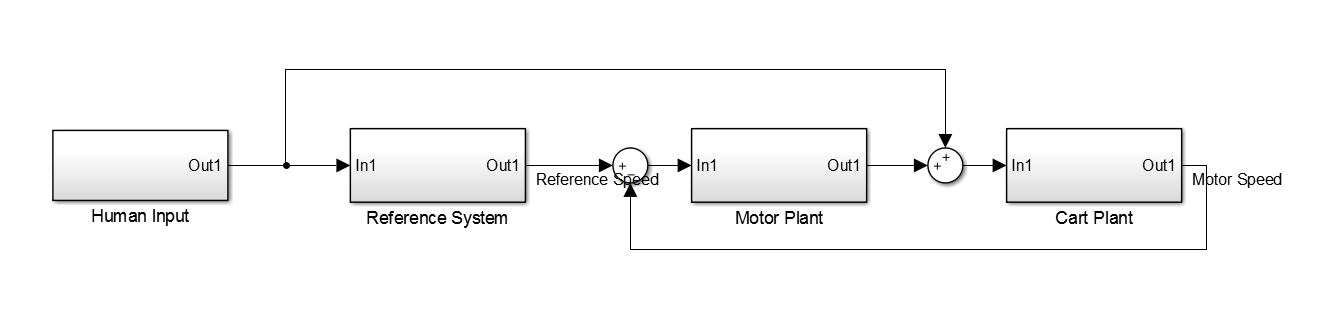
\includegraphics[width=1\linewidth]{Images/ControlLoop}
\caption{Block diagram of the impedance controller. Consists of human input; a reference system with mass, spring and damping parameters from user input; a motor plant and a modeled cart plant}
\label{fig:ControlLoop}
\end{figure*}

Human input for the model has three modes of inputs. Mode 0 is a standard step input with specified amplitude from user input. Mode 1 is a impulse input which has the same amplitude as mode 0, however it has a user defined impulse time. Mode 2 reads experimental data collected from the load cell, it is only used for performance analysis.

The reference system depicts the reaction of a mass-spring-damper setup to a specified input force. A illustrative graph for it is shown in Figure \ref{MSB}. In our model, it is assumed that the spring is always relaxed at the mass's initial position. It also assumes the system has no friction. It will simulate the mass's acceleration, velocity and position based on human input. The simulated speed is then used as reference for the closed loop control system.

\begin{figure}[h]
	\centering
	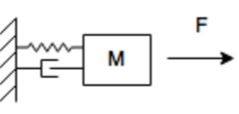
\includegraphics[width=0.5\linewidth]{Images/MSB}
	\caption{Reference System}
	\label{MSB}
\end{figure}

The motor and cart plants are models based on the actual components. Motor plant utilizes a PI controller designed for the system to calculate a control voltage from difference between reference and actual cart speed. The control voltage is then transformed into force applied on the cart through a series of amplifiers and mechanical translations. The cart plant will then calculate the actual speed using both human input force and motor force.

The simulation is used to determine the current, torque and speed requirement for the motor. After running boundary cases from the functional specification map, the peak current and torque requests are found to be no larger than 5A and 2.1N*m respectively, whereas continuous current and torque requests are no larger than 0.6A and 0.2N*m respectively. Samples of simulation results are included in Appendix {{\color{red}\ *}}.

Capability of the PI controller is also found through simulation. A set target speed is used to substitute reference velocity. By running a step response of the system, overshoot of the controller is found to be 18.9\%, whereas the settling time is found to be 0.12s.